\section{Experiment}
\label{sec:experiment}
In this section, we design several experiments to show that our causal embedding 
can not only distinguish between causal and non-causal word pairs but also be used 
in commonsense causal reasoning task.
%To evaluate the property of our causal embeddings, we design several experiments 

\subsection{Dataset}
We extract our causal corpus from a large scale of web texts (~10TB) 
and the total number of sentences matching the causal cues~\ref{tab:cue} is 
nearly 36 million. We lemmatize the sentences using Stanford CoreNLP 
toolkit~\cite{manning-EtAl:2014:P14-5} and filter the stop words 
listed in NLTK~\cite{bird2009natural}. The average length of cause and effect 
span is 8.09 and 8.41 respectively and the size of the vocabulary for cause and 
effect words are 276,749 and 297,920.

Causal relation is but one kind of relation. Our causal embedding 
is capable of distinguishing commmonsense causal relation 
from of other types of relations such as synonym relation.
We prepare two dataset to demonstrate such a property.

\paragraph{\textbf{F}ree \textbf{A}ssociation \textbf{D}ataset (FAD)} 
Created by Nelson~\shortcite{nelson2004university}, 
this dataset contains pairs of words which are correlated but not
necessarily causally related. For example, \emph{flood} may be paired with
\emph{disaster}, \emph{wet}, \emph{overflow} and so on. 
%In Nelson's work, volunteers are given the \emph{cue} 
%word and required to write down the most meaningfully related or 
%strongly associated word, which is named \emph{target}. 
%For example, for word \emph{flood}, volunteers list 
%related words like \emph{disaster}, \emph{drown}, 
%\emph{wet}, \emph{overflow} and so on. 
%Pairs in Nelson's dataset are all correlated but 
%not all of them contain causal realtion.

\begin{table}[th]
	\caption{Sample of human-labeled pairs. Score ranges from 0 to 8. }
	\label{tab:evalset}
	\resizebox {0.5\textwidth}{!}{
		\begin{tabular}{|c|l|c|}
			\hline
			Score & Example & Total \\
			\hline 
			0 & (dance, exercise), (fat, thin), (wine, red) & 1459 \\
			1 & (dance, slow), (risk, take), (drink, water) & 713 \\
			2 & (dance, song), (gun, trigger), (bend, straight) & 552 \\
			3 & (sing, dance), (ice, water), (attack, crisis) & 330 \\
			4 & (dance, step), (book, passage), (stall, delay)& 271 \\
			5 & (dance, grace), (chaos, mess), (fire, help) & 222 \\
			6 & (dance, fun), (fat, diet), (wine, drunk) & 220 \\
			7 & (ice, cold), (battle, blood), (gun, kill) & 129 \\
			8 & (suicide, die), (fireplace, hot), (sun, hot)& 108 \\
			\hline
	\end{tabular}}
\end{table}

We keep the pairs from FAD that match
our vocabulary. Four volunteers then label each pair with a score 
of 0, 1, or 2 indicating if this pair is  non-causal, neutral or
causal respectively. At the end, each pair of words receive a total score
ranging from 0 to 8. In total, there are 4078 such pairs and 
\tabref{tab:evalset} shows some examples.
Because there are only limited causal relations in this dataset, the 
distribution of the scores are skewed toward 0.
We therefore classify pairs with score 0 as negative examples, and those
with score $> 4$ as positive examples. Those with other scores are
discarded. To this end, we obtain 679 pairs from each class.

\paragraph{ConceptNet} 
%As we mentioned in \figref{sec:intro}, 
%ConceptNet contains around 17 thousand causal pairs. 
This is a dataset extracted from ConceptNet, where
each data example contains a positive (causal) pair and a negative 
(non-causal) pair of concepts.
For example, ``punishing'' Causes ``revenge'', and 
``door'' LocatedIn ``house'' form one such example.
Note that concepts can be both words or phrases in ConceptNet,
which is the main difference of this dataset from FAD.

\subsection{Results}
%We use both normalized and unnormalized vectors to calculate the causal strength. 
We evaluate the causal embedding by five experiments on the above two
datasets. Our baseline methods are Word2vec embedding, and CausalNet
from Luo et al~\shortcite{luo2016commonsense}.

We tune the hyperpatameter $\lambda$(Equation~\ref{eq:cs3}) using the experiments above.We perform the three metrics in FAD and results are shown in Figure~\ref{fig:lambda}. 
We also try normalized vectors(i.e. cosine similarity) and unnormalized ones(i.e. dot product).
It shows that we can choose $\lambda$ as 0.6 or 0.8.


\begin{figure*}[th]
	\centering
	%\epsfig{file=causalnet.eps, width=0.6\columnwidth}
	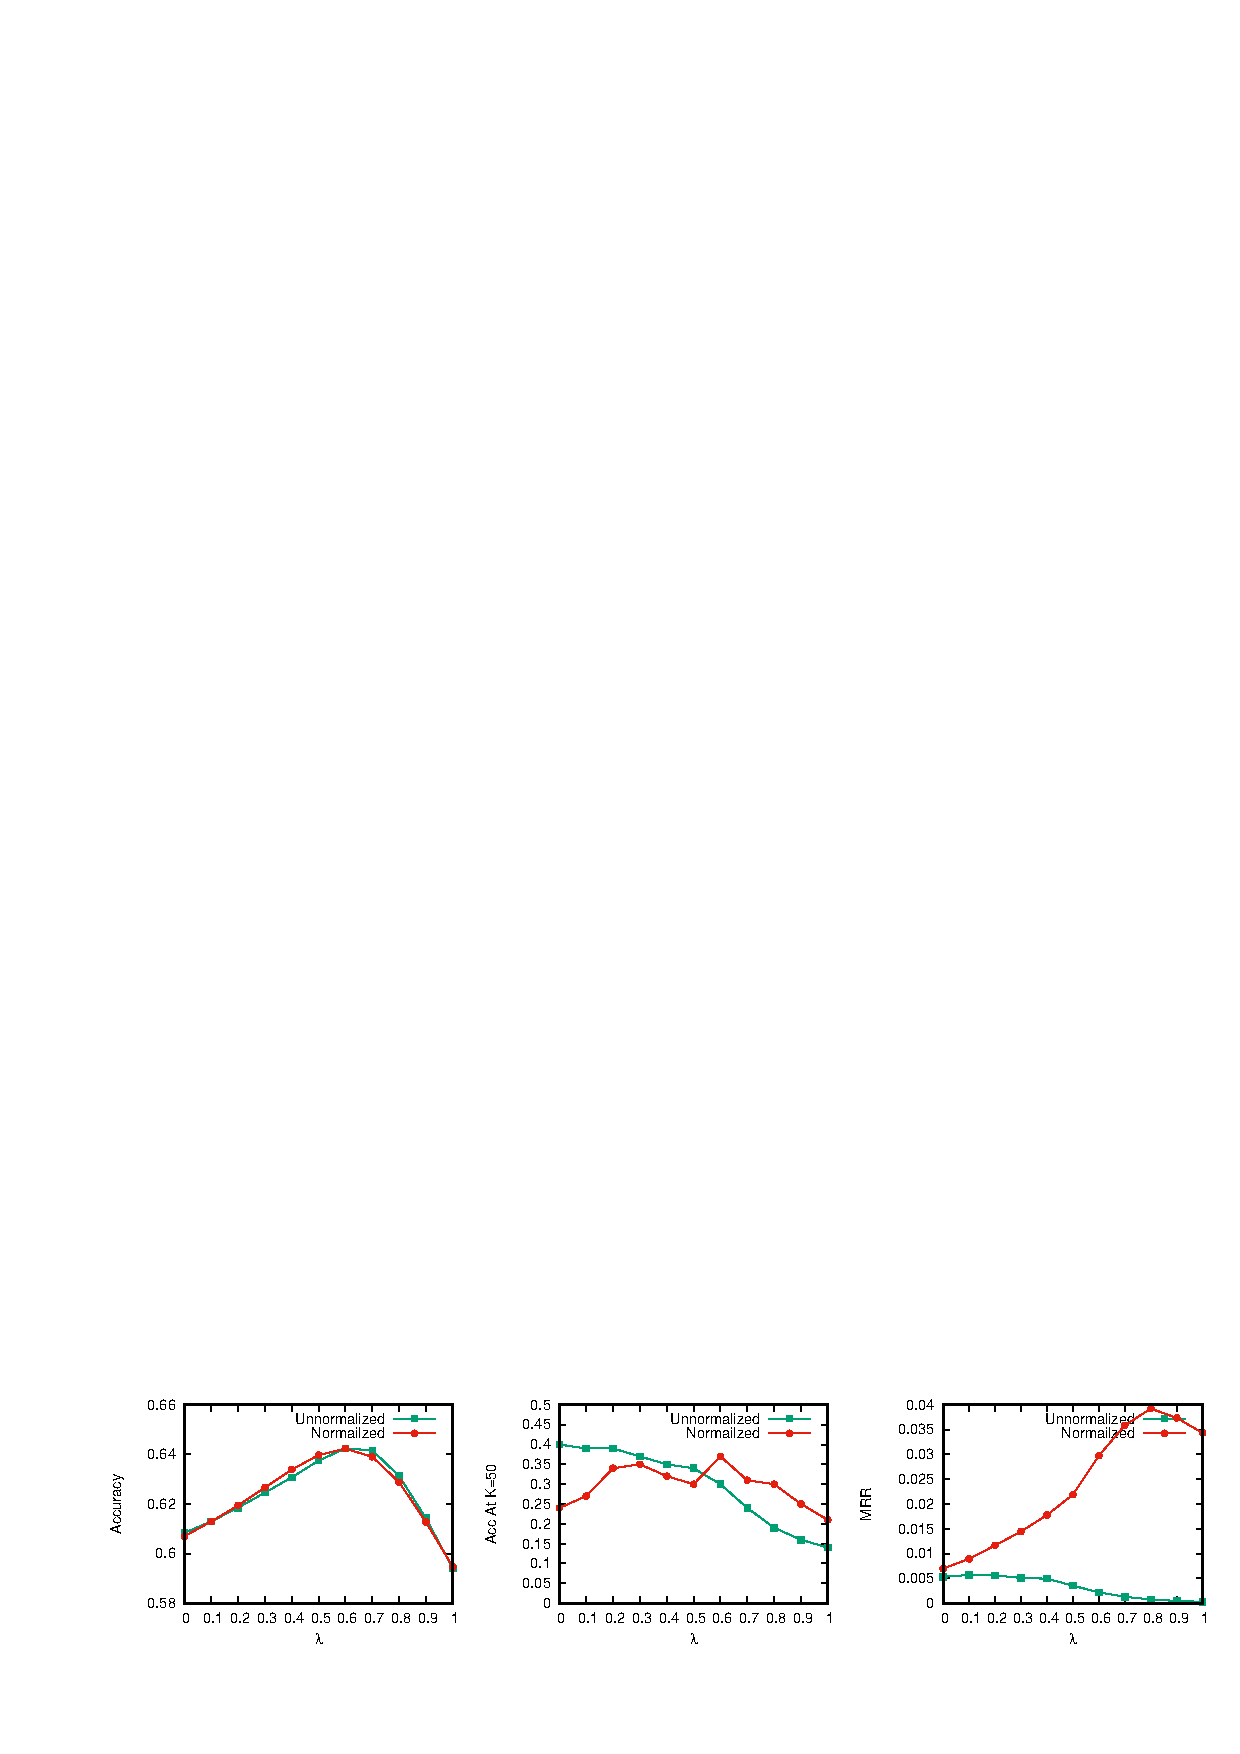
\includegraphics[width=2\columnwidth]{figure/lambda}
	\caption{Evaluation on different $\lambda$s}
	\label{fig:lambda}
\end{figure*}

We then compare our final causal strength with Luo's scores in ConceptNet, results are shown in Table~\ref{tab:conceptnet}

\begin{table}[th]
	%\small
	\centering
	\caption{Result of ConceptNet}
	\begin{tabular}{cc}
		\hline
		Methods & Accuracy(\%) \\
		\hline
		$CS_{\lambda=0.9}$(Luo's best result) & \%  \\
		Causal Embedding with $\lambda=0.9$ & \%  \\
		Word Embedding using Word2Vec & \%  \\
		\hline
	\end{tabular}
	\label{tab:conceptnet}
\end{table}


\subsubsection{Causal Relation or Not?}
Given a pair of words or concepts, this experiment tests the ability
to classify this pair as a causal or non-causal work. For our method
and Word2Vec, we vary the threhold value from 0.1 to 0.9 and plot
the graph in \figref{fig:bin}.

\subsubsection{Ranking of Causal Pairs}
As a ranking problem, in this experiment the competing methods
ranks a given list of word or concept pairs and we compare the rankings
to the gold standard. The results are evaluated using a metric called
``accuracy at $k$''.

\subsubsection{Prediction of Cause or Effect}
In this experiment, we ask the competing method to predict an effect word
given a cause word, or vice versa. Here, Mean Reciprocal Rank (MRR) is used
to evaluate the ranking performance. 

\subsubsection{Causality between Any Two Words}

\subsubsection{Composition of Embedding $C_1 + C_2 \approx E$?} 


%\paragraph{Metric 1: Accuracy of binary classification}
%Causal strength we provided can be used to distinguish postive and negative causal pairs. For example, given pair \emph{(suicide, die)} and \emph{(dance, slow)}, we hope that it is more possible that \emph{$suicide_c$} causes \emph{$die_e$} rather than \emph{$dance_c$} causes \emph{$slow_e$}. For FAD, we pair each positive causal pair with every negative one forming the positive-negative pair. 
%
%\paragraph{Metric 2: Accuracy at $k$}
%We also want to show the  score distribution of the dataset, expecting that the correct causal pairs tend to have high scores. Therefore, we rank the test set of FDA(679+679=1358 pairs) according to their scores and calculate the accuracy at k for the dataset.
%
%\paragraph{Metric 3: Mean Reciprocal Rank} 
%\textbf{M}ean \textbf{R}eciprocal \textbf{R}ank(MRR) is usually used in information retrieval system. In our task, we hope that our scores can recommend proper effect(cause) events given one cause(effect) event. For positive pairs in FAD, we fix the cause side(286 distinct cause words) and search for the closest 1000 effect words. We hope the rank that most possible effect is higher.
% 

%
%\paragraph{Span Size}
%We define the cause and effect span in Eection~\ref{subsec:vec repre} which are the whole span of the half sentence. However, it is more likely that the real cause or effect appears closer to the causal cue. For sentences in Example~\ref{eg:sen}, key event ``flooding'', ``damage'', ``downpour'' are all within 3 words from the pattern. Proper span size can improve our result by removing irrelevant words but also takes the risk of losing the knowledge. 
%
%\begin{figure*}[th]
%	\centering
%	\epsfig{file=causalnet.eps, width=0.6\columnwidth}
%	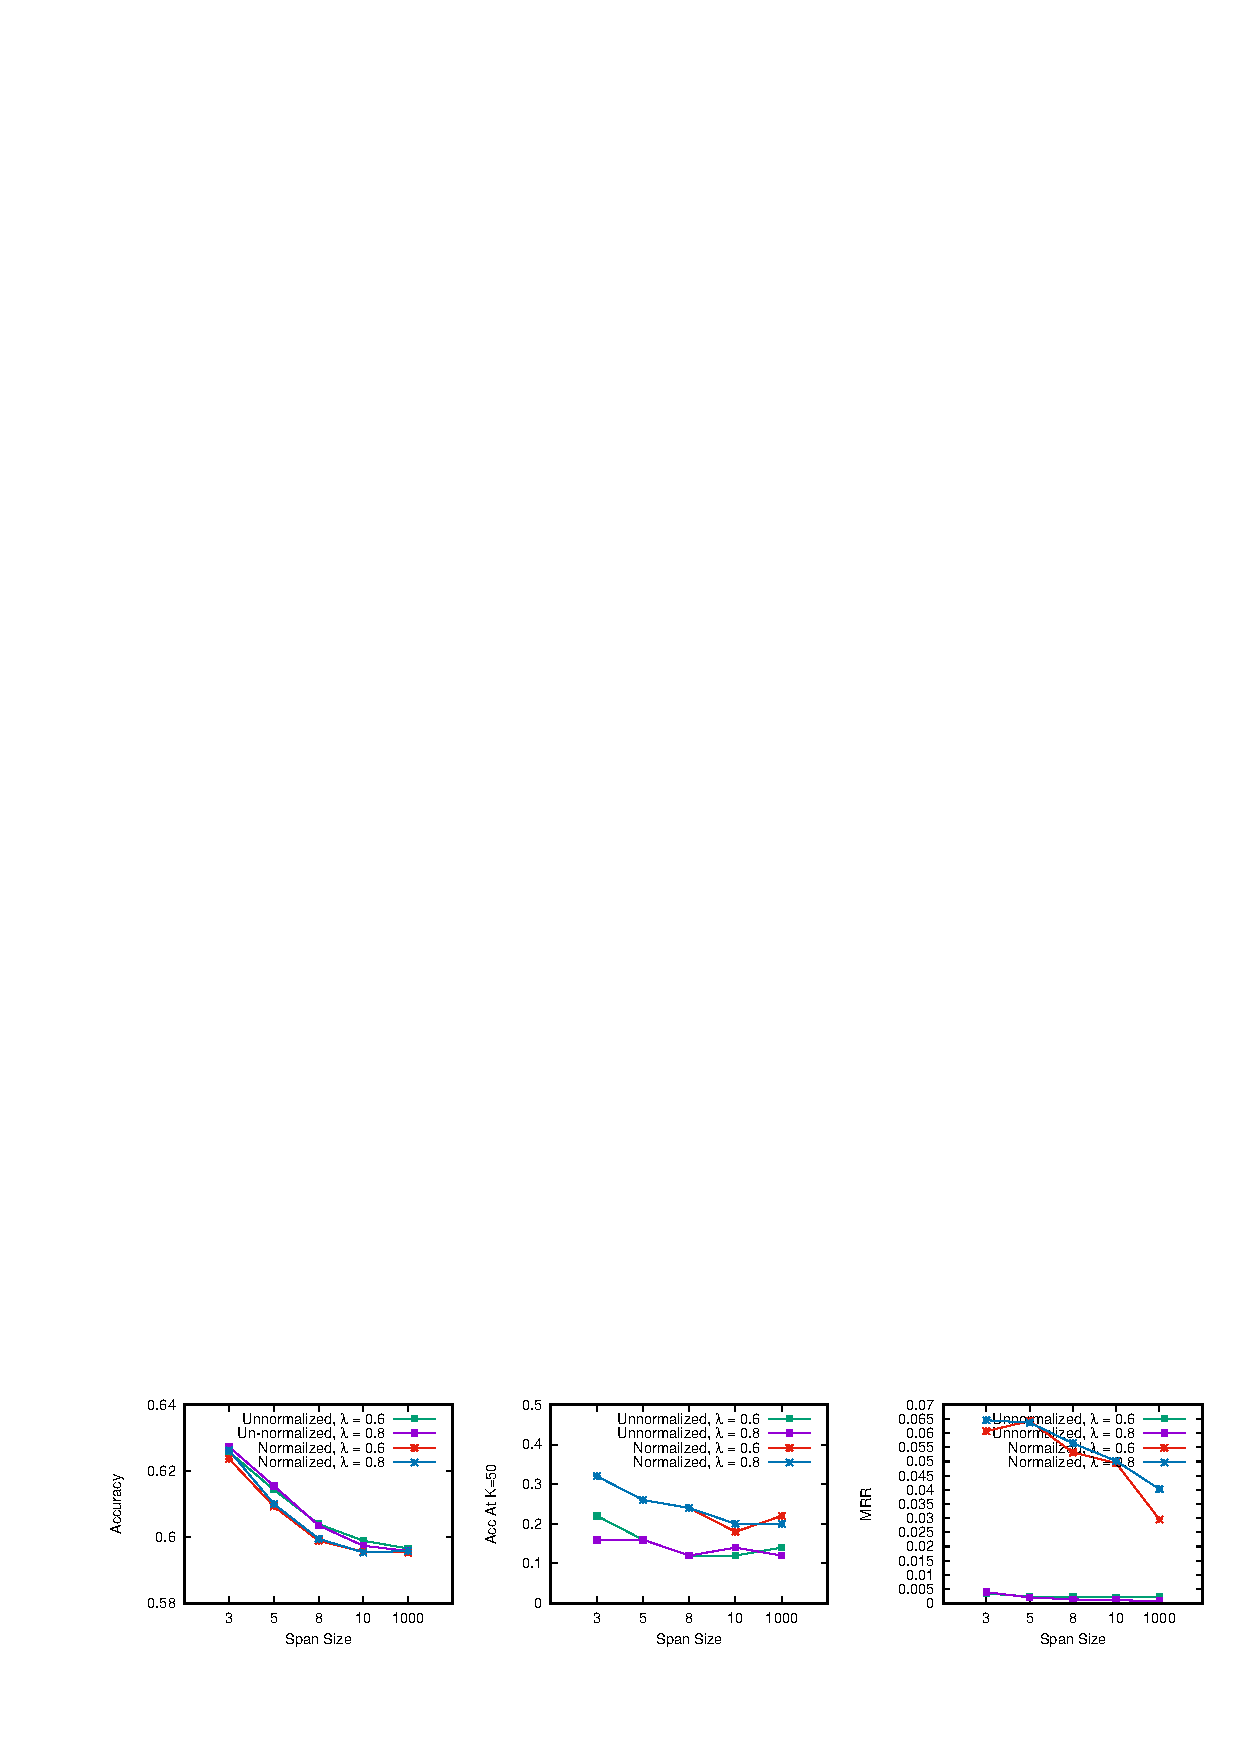
\includegraphics[width=2\columnwidth]{figure/spansize}
%	\caption{Evaluation on different span sizes}
%	\label{fig:spansize}
%\end{figure*}

%\paragraph{Iteration Times}
%As the iteration number increase, the quality of the dataset gets better. Figure shows ....

\subsubsection{Qualitative Results}
\begin{table*}[!ht]
	\caption{Sample of causal pairs}
	\label{tab:qualitative}
	\centering
	\small
		\begin{tabular}{|l|l|l|l|}
			\hline 
			Cauase & Top necessity Effects & Top Effects($\lambda$ = 0.6) & Top Effects of Luo et al. \cite{luo2016commonsense} \\
			\hline
			rainfall & flooding, flood, drought& &roundheaded, litchee, epipactis\\
			accident & fatality, die, death, fatal & & distrait, crippling, aviatrix\\
			virus & hepatitis, infected, viremia&  & ecballium, hominoidea, discase\\
			drown & death, swim, suffocation& & equaphobia, diminutiveness\\
			pregnant & abortion, fetus, baby&& jotunn, pycnanthemum, lopid \\
			\hline 
			\hline
			Effect & Top sufficiency Causes & Top Causes($\lambda$ = 0.6) & Top Causes of Luo et al. \cite{luo2016commonsense} \\
			\hline
			damage & magnitude-5, waterspout& & reliance, tornade, vehicular\\
			happy & love, joy, wonderful, hope& &offend, flag, reproach, goosy\\
			light & illumination, bright, lamp& & air, refractive, phototropism\\
			hurt & feel, break, cheat, love& & dacoity, screwing, padding\\
			die & complication, accident& & complication, accident, sustain\\
			\hline
	\end{tabular}
\end{table*}
We compare our final results with Luo~\cite{luo2016commonsense}'s dataset. The results are shown in Table~\ref{tab:qualitative}.



%\subsection{Application}
%\label{sec:app}
%We apply our causal embeddings on Choice of Plausible Alternatives(COPA)~\cite{roemmele2011choice}, a multiple-choice problems asking for cause or effect given the other side. Below is one example of COPA dataset.
%
%\begin{example}
%	\label{ex:copa}
%	\noindent
%	\begin{itemize}
%		\item[] Premise: \emph{I knocked on my neighbor's door.} What
%		happened as an effect?
%		\item[] Alternative 1: \emph{My neighbor invited me in.}
%		\item[] Alternative 2: \emph{My neighbor left her house.}
%	\end{itemize}
%\end{example}
%
%In this example, we are given the cause side event ``\emph{I knocked on my neighbor's door.}'' and required to choose the more possible effect.
%We solve this problem by two sides.
%
%\paragraph{Sentence-level Solution}
%Since we already have the word embedding for cause and effect roles, we can generate the sentence embedding for premise and alternative by averaging the sum of all words' vectors.
%The causal strength between the two sentences is the dot product of the two vectors.
%
%\begin{equation}
%	CS_{sen}(S_1, S_2) = (\frac{1}{|S_1|}\sum_{c_i \in S_1}{\overrightarrow{c_i}}) \cdot (\frac{1}{|S_2|}{\sum_{e_j \in S_2}\overrightarrow{e_j}})
%\end{equation}
%
%\paragraph{Word-level Solution}
%We can also follow the method used by Luo~\cite{luo2016commonsense}, using the word level causal strength.
%\begin{equation}
%	CS_{word}(S_1, S_2) = \frac{\sum_{c_i \in S_1, c_j \in S_2}{\overrightarrow{c_i} \cdot \overrightarrow{e_j}}}{|S_1|+|S_2|}
%\end{equation}
